\section{Application}
\label{Application}
	\subsection{Information Procurement}
	The main theme of the collected data would concentrate around the topic of Internet Sales Platforms also known as E-Commerce. Several aspects make the topic beneficial for this research. Firstly,  such companies are almost exclusively web-based. It is therefore probable that most of the company's marketing efforts as well as overall news relating to such a firm, would circulate first and foremost in the Internet. Secondly, all company-relevant news are attainable from the web before all other resources. Hence, such news will in all likelihood seep to social media faster than announcements and other stories, which are predominantly covered by traditional media such as television and Newspapers. Therefore, the E-Commerce theme is likely to be widely and swiftly covered on social media, which is beneficial for the purposes of this study, since social media is used as the source of all data.
	
		\subsubsection*{Search Terms}
			The data was collected in the form of relevant Tweets from the Twitter Stream API. A Tweet would be considered relevant if it contained a search parameter related contextually to E-Commerce. The initial efforts were concentrated around the web-store Amazon. \textbf{Amazon} appears to the most fruitful search parameter, in terms of the quantity of Tweets relating to it. Additional search words that were tested were {\bfseries Alibaba, Zalando} and {\bfseries Groupon}, but proved to be impractical due to less data. 
			
			\par
			
			The widespread mention of Amazon in Tweets is somewhat over-inflated due to the extensive use of Amazon gift cards. Amazon gift-cards have become preponderate owing to their variety of uses. A few examples of common practices involving Amazon gift cards are rewarding users for services, such as polls and questionnaires, enticing people to take part in events or groups, and being offered as general rewards in competitions and games. The plethora of uses, facilitates Amazon gift cards to be viewed as a sort of pseudo-currency in the Internet. In turn this means, that Amazon could be mentioned in a Tweet, despite the context only indicating the Gift-card and being completely unassociated to the E-Commerce platform directly. Such Tweets are generally less valuable for the purpose of gaining knowledge about Amazon itself.
		
		\subsubsection*{Collecting the Data}
		\label{sec:collect_data}
			The gathering of Tweets was executed using a program written in the Python programming language for the purpose of this research. All software created for this project is available on \href{https://github.com/burningskies42/Twitter_Analytics}{\textit{GitHub}} \footnote{\url{https://github.com/burningskies42/Twitter_Analytics}}. A wrapper module called \textit{Tweepy}\footnote{\url{http://tweepy.readthedocs.io/en/v3.5.0/}} was implemented for interacting with the Twitter Streaming API. Tweepy is an open source interface, which allows communicating with the Twitters servers and sending queries requesting specific information from Twitter's databases. The interface allows for two main type of queries, \textit{Rest} and \textit{Streaming}. The former scans the servers for information posted on Twitter in the past whereas the latter, as the name implies, connects to an active data stream containing a narrowed down flow of Tweets being actively published by Twitter users. Both types of API's are being offered for free to a certain extent, whereas almost unrestricted versions of the same API are offered as a proprietary fee-based product of Twitter. The free version of the REST API is restricted to looking up Tweets posted in the last two to three weeks. Similarly, the gratis version of the Streaming API is restricted to a fire-hose narrowed down to about 15\% of the total Bandwidth of all current Tweets.
			
			\par
			
			The data units incoming from the Twitter servers are sent as JavaScript Object Notation (JSON) strings. JSONs are structured hierarchically, which allows for embedding other JSON objects in them recursively. This makes JSON beneficial for Tweets, since it allows multi-level storage of Tweet properties and objects. For example, one of the JSON objects integrated in each Tweet JSON is the USER object for the Tweet-poster. A USER object, a JSON by itself, contains all relevant data for a Tweeter account. The USER object in turn contains all data publicly available in Twitter about a Twitter account such as, location, date of registration, homepage etc. An additional object of interest is the ENTITIES JSON object, which contains all outside references from the Tweet's text such as, URLs, Multimedia, References to other Tweets or other users. 
			This structure greatly eases the analysis of a Tweet and its features, since most of the necessary data is available from the Tweet itself and no further queries about the Tweets and its posting-user are necessary.
			\par
		{\LARGE \color{red}
			elaborate about stages of data collection:
		} \\ 
		{\color{red}
			1. Initial data: full of duplicates\\
			2. Filtered data - fewer duplicates and Spam, but still rather very one-subject-centered. Leads to overfitting when classifying \\
			3. still untried - collect up to x (~400) Tweets per day, for a duration of ~ 2 weeks
		}
		
		\subsubsection*{Data cleansing}
			It was observed that numerous Tweets were being posted more than once and in several occurrences even hundreds of times. These duplicates were being primarily posted by bots, as was evident from a short observation of user profiles belonging the Tweets original posters. Evidently, additional effort was being made by the programmers of the bots to try and mask them by slightly altering the content of the Tweets, or the user account. This was usually done by changing or adding characters to the text, which carry no lingual significance in themselves. Moreover, in furtherance of increasing the bots' credibility as an actual people, often times entire nets of such bot could be observed, wherein the bots would maintain friendship and following connections among themselves. An example is shown in figure \ref{fig:twitterbot}. This in turn, increases the amount of \textit{friends} and \textit{followers}, further contributing to their guise of real human users of Tweeter. Upon closer observation, such accounts reveal their true essence, since most of the content propagated by them is commercial in nature and is repeated verbatim time and again across many of the related accounts \textit{followers} and \textit{friends}. For this reason, it is safe to assume that no actual people are behind these accounts. 
		\par
		
		\begin{figure}[h]
			\centering
			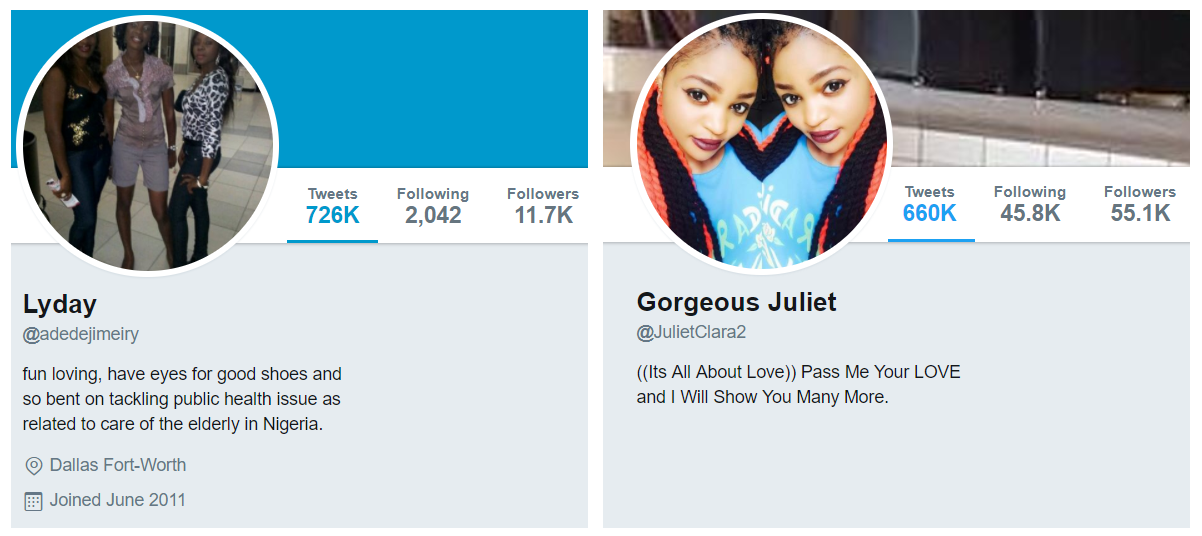
\includegraphics[width=0.8\textwidth]{twitterbot.PNG}
			\captionsetup{width=0.8\textwidth}
			\caption[Fake Twitter Accounts]{Twitter accounts, which present themselves as actual people}
			\label{fig:twitterbot}	
		\end{figure}
		
		\newpage
		\noindent
		Several precautions were undertaken to try and filter out such bots. A passive precaution which was implemented, was blacklisting users, which had priorly been observed posting Tweets, which were verbatim copies of other Tweets within the same query. The suspected users were added to a suspect database and content originating from them was ignored in future queries. Another action undertaken with the same purpose in mind was a retrospective cleanup of the collected Tweets, based on their content similarity. After closing a collection query, a maximum similarity measure for each Tweet in relation to all other recorded Tweets was calculated using a simple rule. Following, Tweets which were found to have a maximal similarity score to other previously captured Tweets  higher than a predetermined threshold were classified as non-unique copies and were disregarded. As a measure of similarity, the S\o rensen-Dice coefficient \cite{sorensen1948method} was implemented  using the \textit{SequenceMatcher.ratio()} function from the difflib Python module. The coefficient is demonstrated in figure \ref{fig:sorenson_dice} where $|X|$ and $|Y|$ are the numbers of elements in given Tweets X and Y accordingly. A higher $ QS_{XY} $ value indicates larger conformity between the $ X $ and $ Y $ groups, and ranges from 0 (completely different) to 1 (identical).
		A round of cleanup using this procedure would usually reduce a data set by from one quarter and up to one half of its original size.
		
		\begin{figure}[h]
			\begin{center}
				$QS_{XY} = \dfrac{2|X\cap Y|}{|X|+|Y|},$ \hspace{10pt}  $QS_{XY} \in [0:1]$
			\end{center}
			\caption{S\o rensen-Dice coefficient}
			\label{fig:sorenson_dice}
		\end{figure}
		
		\newpage
		
	\subsection{Building Feature-Sets}
	\label{build_features}
	Once a list of labeled Tweets is obtained, the next stage is constructing a feature-set to be later passed on as input for training an ML Classifier. The features contained if the feature sets describe certain aspects and characteristics of a Tweet and its owner. Two main approaches to feature sets are \textit{Word-Based} also often called \textit{Bag-of-Words} and \textit{Descriptive}. A further modification on \textit{Bag-of-Words} is \textit{N-Grams}.
	
		\subsubsection{Word-Based Features}
			The former approach simply converts the entire text corpus to a frequency charts of all the words contained within. Words are then selected to act as features in incoming data, which is to be classified. The features are hence a variable list (usually of several thousands in length), where each variable is a boolean representation, indicating the presence or absence of a certain word. Usually the words undergo preprocessing as is common in Natural Language Processing prior to being used as features. The corpora are segmented to lists of words, often omitting articles, proposition and punctuation. Such grammatical structures are critical in human speech and written form in order to convey ones meaning clearly and explicitly, however for the purposes of more ambiguous classification as in our case, such nuances are avoided for the sake of simplicity. Words are then \textit{stemmed} or \textit{lemmatized}, meaning their are reverted to their grammatical stem - dropping all prefixes and suffixes. This eases the enumeration of words, since it is preferable that the same words in different inclinations would be counted as the same. For example, the word pair \textit{eating} and \textit{ate} would be reverted to their stem \textit{eat}, as well as \textit{apple} and \textit{apples} would be considered as one and the same. Finally, words would be assigned their part of speech (noun, verb, adjective ..) and could be either ignored or incorporated into the feature set, according to the conceived importance of a given part of speech.
		
		\subsubsection{N-Grams Features}
			A development on the Bag-of-Words concept. Using this approach, sequences of $ n $ words are extracted instead of single words and used as features. Such an approach has the added benefit of preserving some of contextual meaning of the text as well as discovering reoccurring phrases. This would prove even more beneficial is scenarios, in which the classification would be between positive and negative intonation, such as opinions and reviews. A down side to this method, is that much more feature are created therefore increasing the computational complexity. For example, using standard Bag-of-Words approach on the sentence "the movie was not great" results in 5 features \{the; movie; was; not; great\}. When applying N-Grams of sizes 2 to 5 on the same sentence, results in 10 features as seen in table \ref{table:ngrams}.
			
		\begin{table}[h]	
			\begin{center}
				\begin{tabular}{||c l||} 
					\hline
					N &   possible N-Grams  \\ 
					\hline\hline
					2 & the movie; movie was; was not; not great  \\
					\hline
					3 & the movie was; movie was not; was not great \\
					\hline
					4 & the movie was not; movie was not great \\
					\hline
					5 & the movie was not great \\ [1ex] 
					\hline
				\end{tabular}
			\end{center}
			\caption[N-Gram Example]{Possible N-grams of size 2 to 5 }
			\label{table:ngrams}
		\end{table}
		
		
		\subsubsection{Descriptive Features}
			The latter approach mentioned is based on a more generalized view of the Tweet. Instead of concentrating on the actual textual content, other non direct properties are observed. Descriptive features are aimed at describing the Tweets implicit properties, such as attitude, sentiment, seriousness and trustworthiness. These features detect the presence of different symbols, their frequency and consecutiveness. Additionally, unlike the Word-Based approach, non-textual objects such as multimedia, links and mentions of other users and Tweets are also taken into account. Furthermore, features of a Tweets' owner are also included in the input. Since Tweeter's API provides a complete user profile incorporated inside the Tweet data object itself, constructing features describing the user is done simultaneously to features describing the content of the Tweet itself. This approach might be viewed as an \textit{indirect} one, since less obvious properties of the Tweet are used to characterize it.
			\par
			Descriptive features could be segregated into two distinctive groups. The first tier is text-based features. As the name suggests, these features will mostly denote the presence or lack of specific characters such as emoticons and signs in the Tweets text. Whether a Tweet contains combinations or sequences of certain symbols as well as ratios defining the text also befit this category.
			\par
			The second tier of features describe any special \textit{Entities} (Tweeter's nomenclature) contained within a Tweet. \textit{Entities} refer to non-textual contents of a Tweet, such as media (in form of pictures, audio or video), URL's linking to external websites, mentions or Retweets (referring to other Tweets or to Tweeter user profiles) and finally Hashtags. A word or phrase preceded by the Hashtag symbol \textbf{\#} indicates an association of web content (such as a Tweet or other micro-blogging post) to a specific theme. These could be an event, news, gossip or any other tidbit \cite{dict_Tweet}. Hashtags are used primarily to simplify looking up Tweets or other social media content by technically associating them with the \textit{hashtagged} topic.
			
	\subsection{Training Classifiers}
		Several configuration are to be applied when training the different classifiers, in the interest of quantifying and measuring the quality of classification. Hence, the size of the datasets used for training will vary, to observe the relation between set size and classifier accuracy. Additionally, different amounts of features should be tested, to determine whether accuracy grows linearly as the number of features increase or rather converges after some threshold. Furthermore, the training duration is to be measured to determine effectiveness of training as a time function.
		
		\par
		
		The different classifiers are grouped according to their designation and type as discussed in \hyperref[classifer_types]{section 3.2}. Additionally, another classifier type is one, which incorporates all previous classifiers and classifies with a majority vote. This classifier will be referred to as Vote Classifier. An apparent drawback of the Vote Classifier, is the classification duration which will be as long as the sum of classification durations of all its components.
		
		